\section{Boomerang Overview}
At its heart, Boomerang is a peer-to-peer mixnet that can be leveraged by any anonymizing coin, such as Zerocoin, to provide anonymity analogous to Tor without the same side channel vulnerabilities. The main idea is to hide the source or origin from which transactions are introduced into the network. To do this, we integrate traditional mix networks into the peer-to-peer Bitcoin network such that new transactions which are to be broadcasted must first pass through a series of mixes (which are actually other participating Bitcoin users) through the network so as to obfuscate the originating network address. Functionally, this is no different from Tor. However, Boomerang has several important distinctions that make it unique with respect to onion-routing techniques like Tor:
\begin{enumerate}
	\item Transaction anonymity increases \emph{for every participant} when more people use Boomerang messages to broadcast transactions - everyone is therefore incentivized to use Boomerang. 
	\item Involuntary mixing delays mitigate timing-based side channel attacks that can be leveraged to deanonymize clients using Tor. 
	\item Boomerang messages are enhancements to the Bitcoin protocol, rather than a means for anonymizing point-to-point TCP connections, as is done with Tor. 
\end{enumerate}

The main design goals of Boomerang are as follows:
\begin{description}
	\item[Sender anonymity]: \\A node achieves \emph{sender anonymity} if a node cannot be (uniquely) identified, or linked, to a particular transaction that is broadcast at the end of a Boomerang circuit (see Section \ref{sec:design}) \cite{AnonymityTerms}. 
	\item[Fault-tolerance via redundancy]: \\Compromised or mobile nodes should not lead to significant delays in transaction introduction or compromise mixnet deadlocks.
	\item[Performance]: \\Nodes in the network should incur minimal overhead from using Boomerang messages while maximizing their anonymity.
\end{description}

We now provide a brief overview of how Boomerang is used by clients for transaction broadcast anonymity; A complete description of the protocol is provided in Section 4. To broadcast a new transaction $T$ using Boomerang, a client $C$ first creates a set of $W$ individual mixing circuits of length $D_1,D_2,\dots,D_W$, where $W \geq 1$ and $D_i \geq 2$. Let $K = \sum_{i=1}^WD_i$ be the total number of nodes selected as mixing services for the circuits. With knowledge of the public keys for each of the $K$ nodes, $C$ then wraps $T$ in $D_i$ layers of encryption for each circuit $i = 1,\dots,W$. Each layer of encryption also includes a forward pointer to the subsequent hop in the circuit so that decrypting nodes may forward the transaction to the appropriate location, or broadcast the plaintext transaction $T$ if they are the last hop in the circuit. 

As is standard with traditional mix networks \cite{Chaum81-Mix}, each nodes will only forward wrapped transactions after it has accumulated a certain number of transactions from other nodes. For this reason, to avoid network deadlock, we require that ``cover traffic'' be circulated throughout the network to keep traffic moving smoothly, similar to the cover traffic used in the Tarzan mix network \cite{tarzan}. Furthermore, this cover traffic must encoded such that it appears indistinguishable from legitimate encrypted transaction messages. To solve this problem, Boomerang cover traffic messages \emph{are legitimate transaction encryptions}, with the exception that the last ``hop'' of the ``circuit'' for these messages is the same client $C$ that generated them in the first place. Thus, these dummy transaction messages will be circulated throughout the network and ultimately be routed to $C$, who can then easily check that they generated the transaction and discard it (or send out another dummy message). The circular nature of this cover traffic, which is shown by the red trajectories in Figure \ref{fig:boomerang_net}, is the inspiration for Boomerang's name.

\begin{figure}[ht!]
\begin{center}
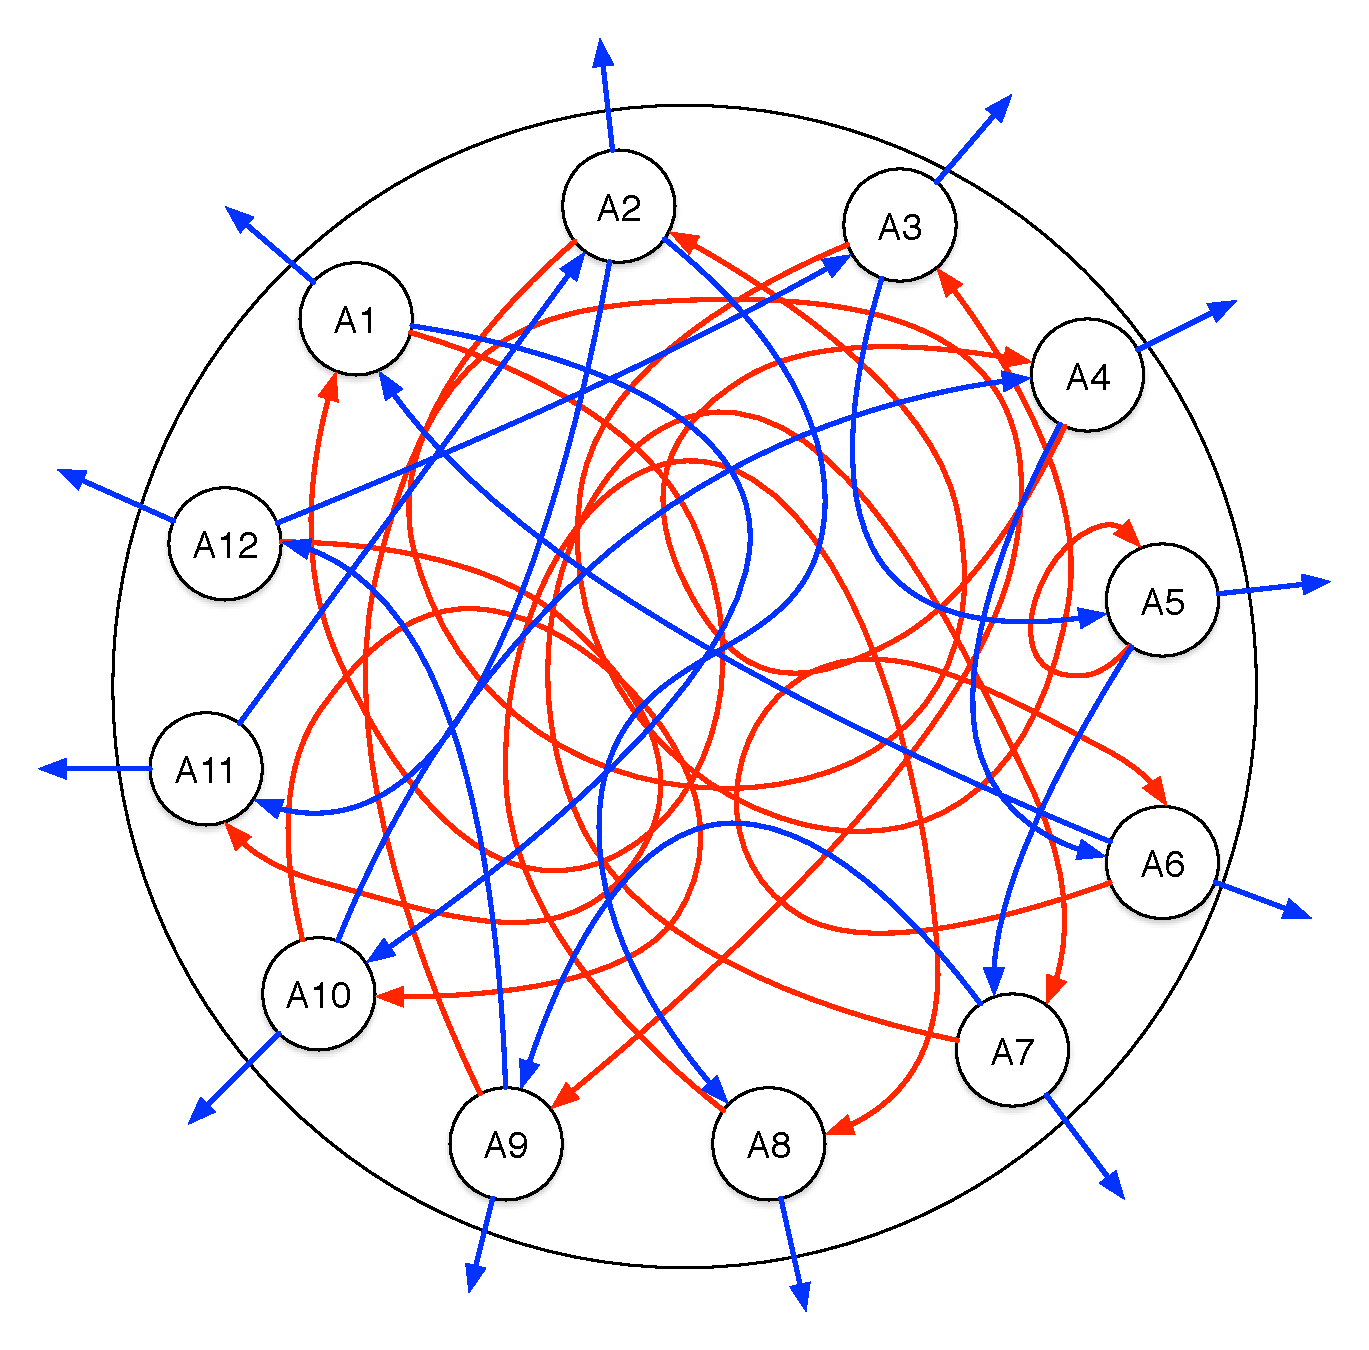
\includegraphics[scale=0.25]{./images/boomerang_net.pdf}
\caption{TODO}
\label{fig:boomerang_net}
\end{center}
\end{figure}

Given this short description, there are many important engineering problems to solve in order make Boomerang feasible in practice, such as public key distribution and usage, prevention of self-induced denial-of-service attacks, and the overconsumption of network resources. We describe solutions to all such problems in Section 4, and include a preliminary performance analysis of the Boomerang technique (based on analytical modeling and simulations) in Section 5. 
